\chapter{Phenomenological study of Run1 four top quark production cross-section limits}
\label{c:pheno}

The 95\% CL upper limit placed on the production of four top quarks at $\sqrt{s}=8$~TeV can be used to place constraints on various physics models. One particular model which is described further in $<theory>$ is a simplified model of NMSSM in which a new particle, the sgluon, arises. The results of the search in the single lepton channel in Chapter~\ref{c:Run1} are used alongside a search for new physics in the same-sign dilepton channel at $\sqrt{s}=8$~TeV~\cite{Chatrchyan:2013fea}, which also places limit on SM four-quark-production, to place constraints on the mass and coupling of the sgluon. The author personally made contributions to reinterpreting that latter search and hence it will be primarily discussed in this thesis. Full details of the combined analysis and particularly the reinterpretation of the single lepton analysis can be found in~\cite{Beck201548}.

\section{A simplified model for describing top-philic sgluons }
$<$\emph{to be completed after theory section is written}$>$
\begin{figure}[h!]
\centering
    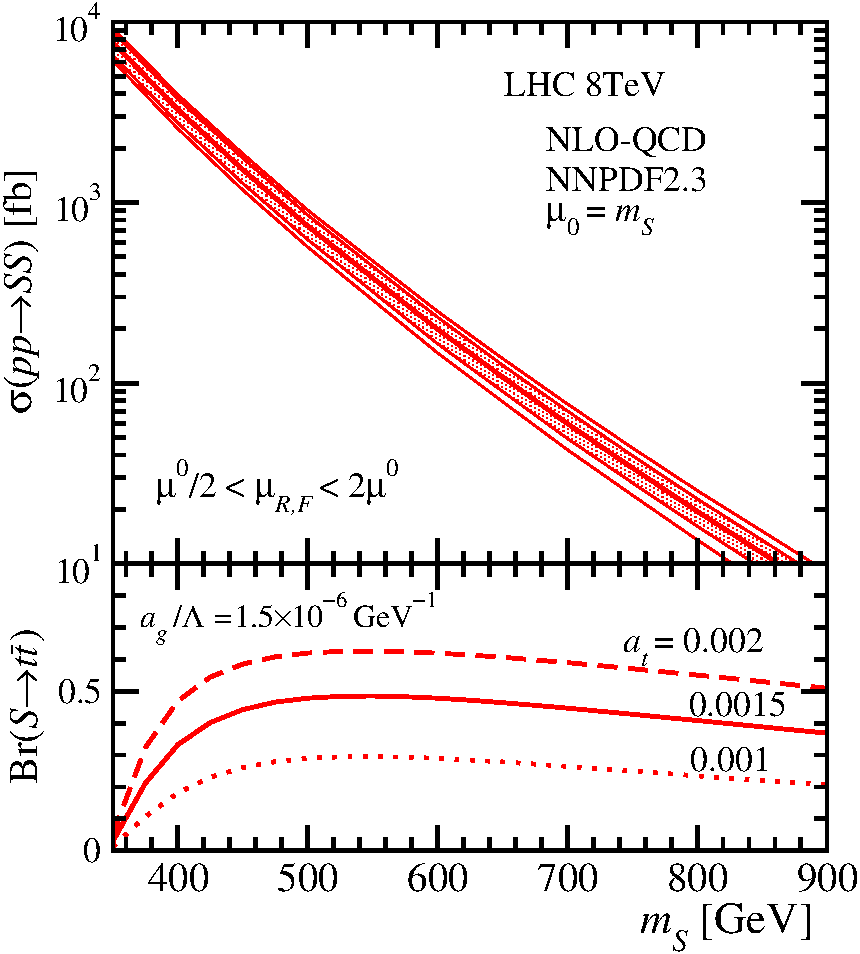
\includegraphics[width=0.7\textwidth]{images/Pheno/xsec.pdf}\\
    \caption{caption}
    \label{fig:sgluonxsec}
\end{figure}
\section{Reinterpretation of same-sign dilepton channel}

The analysis by CMS of the same-sign dilepton channel at $\sqrt{s}=8$~TeV~\cite{Chatrchyan:2013fea} utilises the entire 2012 dataset of proton-proton collision of 19.6~\fbinv. The analysis is a collection of counting experiments that contain at least two same sign leptons and a number of jets. There are 28 signal regions which are categorised in \njets, \nbtags, \HT, \MET and require the leptons to satisfy $\pt>20$~GeV and$|\eta|<2.4$. Signal region 28 (SR28) was chosen to reinterpret as it closely corresponds to the \tttt signature and it can be fully emulated using the parameterisations of selection efficiency given in the paper. It is not possible to combine the results from multiple signal regions without knowledge of the correlation of the uncertainties on the background. 

The efficiency curves for reconstructing an object in the detector given generator-level information are shown in Fig.~\ref{fig:effGraphs} for:
\begin{itemize}
\item The reconstruction of jets with respect to generator-level jet \pt 
\item The b-tagging of b-quark jets by the CSV algorithm with respect to generator-level jet \pt
\item The reconstruction of \HT with respect to generator-level \HT, $\varepsilon_{H_T}$
\item The reconstruction of muons and electrons with respect to generator-level lepton \pt
\item The reconstruction of \MET with respect to generator-level \MET, $\varepsilon_{\MET}$
\end{itemize}

\begin{figure}[ht!]
\begin{center}
% \subfloat{
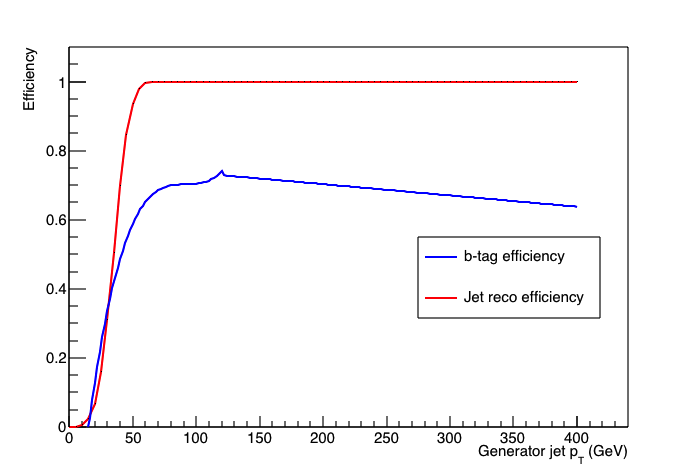
\includegraphics[width=0.49\textwidth]{images/Pheno/BTagEff.png}
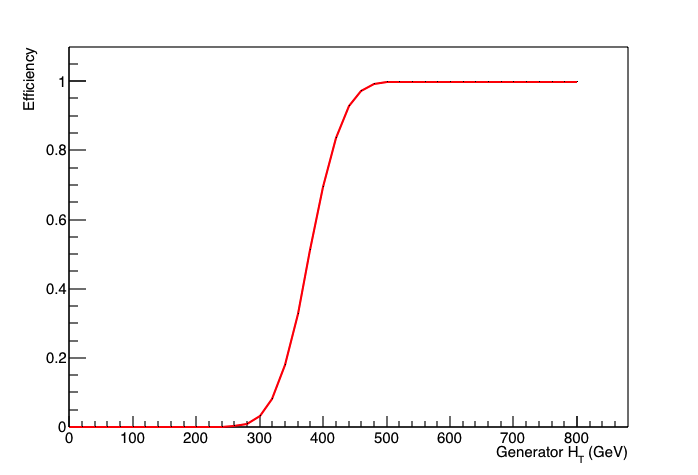
\includegraphics[width=0.49\textwidth]{images/Pheno/HTEff.png}\\
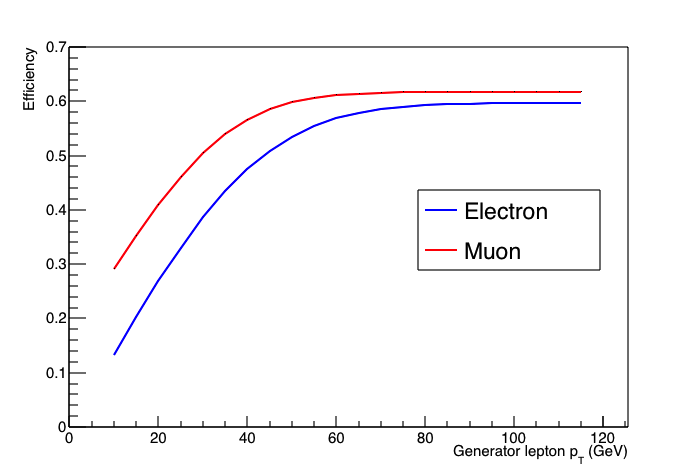
\includegraphics[width=0.49\textwidth]{images/Pheno/LeptonEff.png}
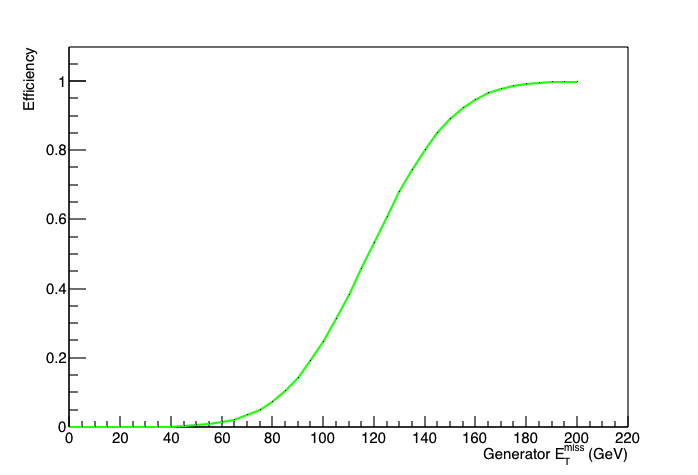
\includegraphics[width=0.49\textwidth]{images/Pheno/METEff.png}
% }
% \hspace{0.2cm}
\end{center}
\caption{Selection efficiencies for the reconstruction of jets and for b-tagging b-quark jets (top-left), for reconstructing \HT (top-right), for reconstructing muons and electrons (bottom-left) and for reconstructing \MET (bottom-right)}
\label{fig:effGraphs}
\end{figure}

The requirements of SR28 are \njets$\geq4$, \nbtags$\geq2$, \HT$>400$~GeV, \MET$>$120~GeV and two same-sign leptons with \pt$>20$~GeV and $|\eta|<2.4$. Events which contain any additional leptons which form an opposite-sign-same-flavour (OSSF) pair with one of the signal leptons is vetoed if the invariant mass of the OSSF (M$_{\ell\ell}$) is either M$_{\ell\ell}<12$~GeV or $76<$M$_{\ell\ell}<106$~GeV. This is to replicate the veto in the CMS search for events which may contain a low mass bound state or a Z boson.

The efficiency, $\varepsilon_{\geq\text{2b-tags}}$, can be calculated using equation~\ref{eqn:2btags} along with the probability, $P_{i}$, for reconstructing a b-jet. $P_{i}$ is the product of the probability to reconstruct a jet$_{i}$ and to tag it as b-jet which can be determined from the parameterisations of the curves Fig.~\ref{fig:effGraphs} (top-left). A uniform efficiency for light quarks to be tagged as b-jet of 1\% is included.


\begin{equation}
w(\geq2~b~tags) = 1 - w(0) - w(1)
\label{eqn:2btags}
\end{equation}

\begin{equation}
w(0) = \prod_{i} ( 1 - P_{i})
\label{eqn:0btags}
\end{equation}


\begin{equation}
w(1) = \sum_{i}\left[P_{i}\prod_{j} ( 1 - P_{j})\right]~;~j\neq~i
\label{eqn:1btags}
\end{equation}

The efficiency for obtaining one same-sign dilepton pair in an event, $\varepsilon_{\geq1 \text{SS2L}}$ can be obtained by using Eq.~\ref{eqn:al1} where $w(\geq2~positive~leptons)$ and $w(\geq2~negative~leptons)$ can be calculated using~\ref{eqn:2btags} along with the probabilities from the parameterisation of the muon and electron efficiency curves in Fig.~\ref{fig:effGraphs} (bottom-left).

\begin{equation}
w(\geq1~SS dilepton pair) = 1 - w(\geq2~positive~leptons) - w(\geq2~negative~leptons)
\label{eqn:al1}
\end{equation}

From the derived efficiencies for obtaining a specific \HT and \MET per event as well as $\geq2$~b tags and $\geq1$~SS dilepton pair, an overall event weight can be calculated using equation~\ref{eqn:phenoWeights}.

\begin{equation} \label{eqn:phenoWeights}
  w_{\rm event} = \varepsilon_{H_T} \times  \varepsilon_{\MET} \times
    \varepsilon_{\geq\text{2b-tags}} \times \varepsilon_{\geq1 \text{SS2L}} \ ,
\end{equation}

\section{Simulation of sgluon events}
The \MGfive software package was used to simulate sgluon pair production with exclusive decays to top quarks at $\sqrt{s}=8$~TeV. \PYTHIAsix was used to perform the hadronisation. The jet clustering was performed using the \antikt clustering algortihm in the \FASTJET package with a cone radius of R$=0.5$ and \pt$>5$ which is consistent with the CMS analysis.

A sample of standard model four top quark events was also simulated using \MGfive and \PYTHIAsix. A signal efficiency for these events passing the SR28 selection was $0.6\%$ which can be compared to the $0.49\%$ signal acceptance found in the CMS analysis. These two numbers are agree within the $30\%$ uncertainty quoted for the analysis.

Sgluon events were simulated for a number of sgluon mass points, $m_{S}$, between $350 \geq m_{S} \geq 1000$~GeV and in the range of coupling to the top quark, $\alpha_{t}$, of $0.5 \times 10^{-3}\geq \alpha_{t} \geq 5 \times 10^{-3}$.

\section{Analysis}

Using equation~\ref{eqn:phenoWeights} one can obtain the correctly weighted number of events which pass the selection and hence the signal efficiency for each sgluon ($m_{S},\alpha_{t}$) point. The number events which would be found in the CMS analysis are obtained using Eq.~\ref{eqn:equivEvents}.

\begin{equation}
n^{S}_{events} = Signal~Efficiency\times cross~section \times SGKfactor \times \mathcal{L} \left(\times coupling reweight\right)
\label{eqn:equivEvents}
\end{equation}

\fixme{Compare to actual events found by CMS using CLS method}

\section{Results}
\fixme{Dilepton analysis better}



\begin{figure}[h!]
\centering
    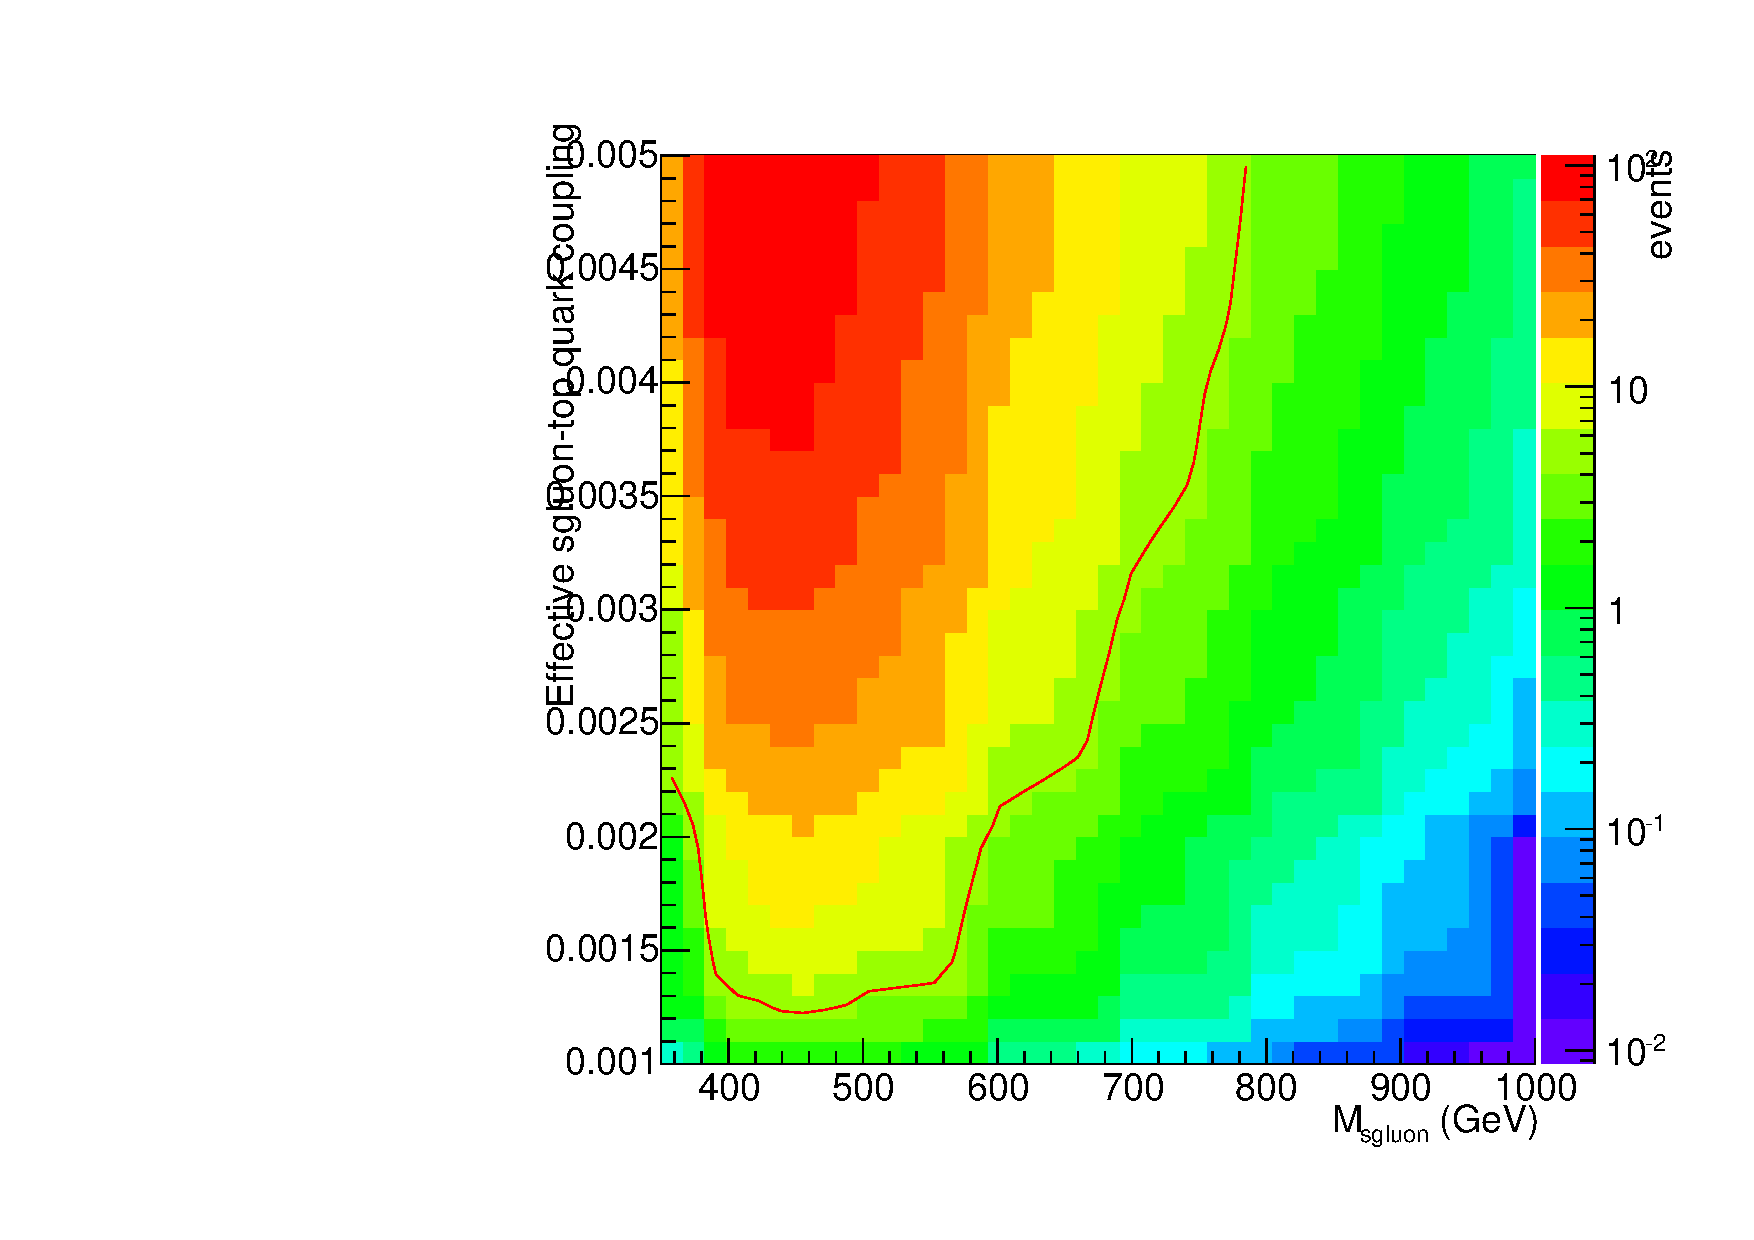
\includegraphics[width=0.7\textwidth]{images/Pheno/SG_nEvents2D.pdf}\\
    \caption{caption}
    \label{fig:dilep2D}
\end{figure}

\begin{figure}[h!]
\centering
    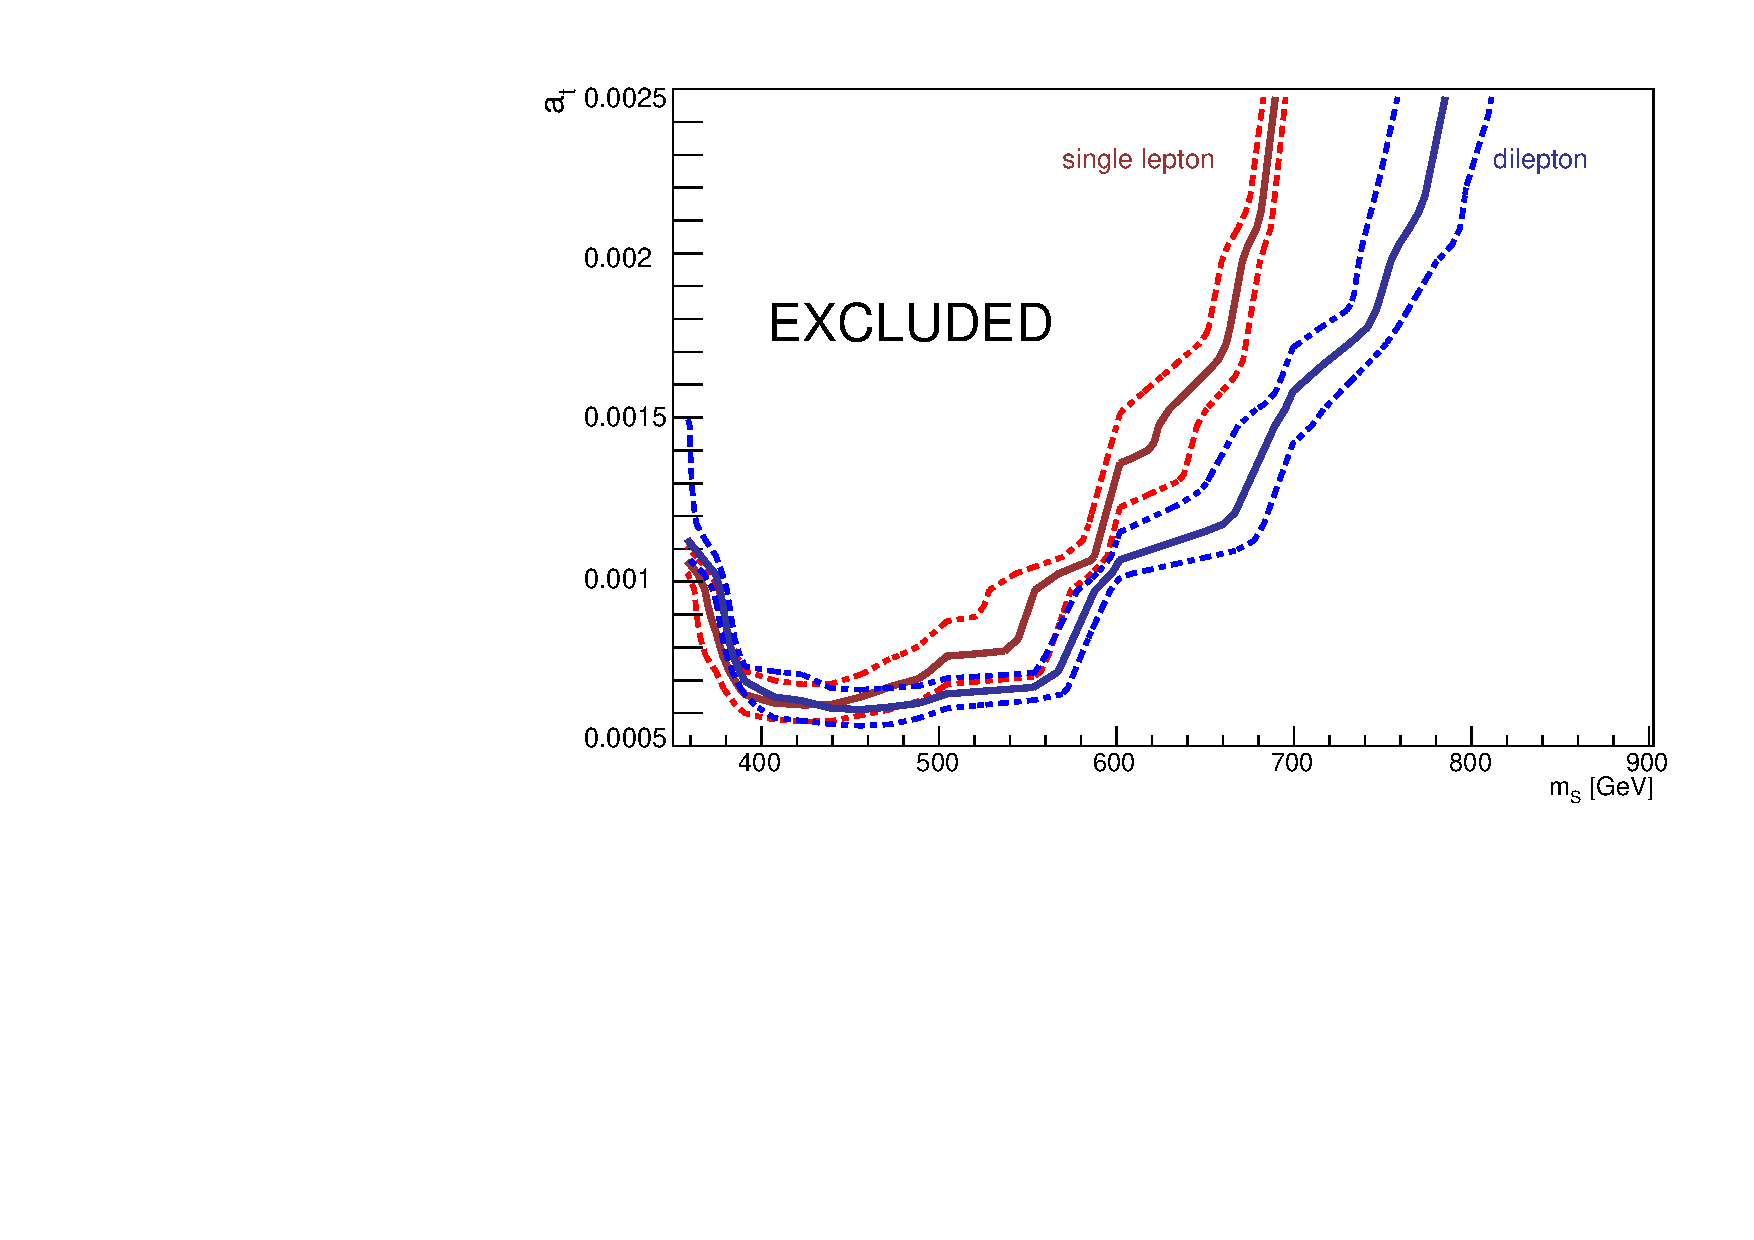
\includegraphics[width=0.9\textwidth]{images/Pheno/exclusion_agVariations.pdf}\\
    \caption{caption}
    \label{fig:sgluonExclusion}
\end{figure}


